\section{Integer programming model}
\label{sec:model}
\TODO{Write introduction to the model}
We will use the definitions $\V$ and $\E$ from page~\pageref{eq:graph} and
definition of $\D$ from page~\pageref{eq:dir} quite extensively in this
section. Every parking space has a status. All possible node statuses are
described in~\autoref{tbl:statuses}. We denote the set of all node statuses
as~$\W$.

\begin{table}
    \begin{center}
        \begin{tabular}{| c | c |}
            \hline
            Status & Meaning \\
            \hline
            \stat{e} & Parking space is empty.\\
            \stat{r} & There is robot on the parking space.\\
            \stat{i} & There is a car with label $i$ in
            the parking space.\\
            \stat{ri} & There is a car with label $i$ and a robot is under it.\\
            \stat{ir} & There is a robot carrying the car with label $i$.\\
            \stat{lft} & There is a robot in the process of lifting a car.\\
            \stat{drp} & There is a robot in the process of dropping a car.\\
            \hline
        \end{tabular}
        \TODO{make this table nice}
        \caption{We list all possible statuses of parking spaces with their
            descriptions. Note that $\stat{i} \in \{0,\ldots,K-1\}$. So when
            there is a robot carrying car with label 2, the status should be
            \stat{2r}, not \stat{ir}.}
        \label{tbl:statuses}
    \end{center}
\end{table}

When a object moves from node~$u$ to an adjacent node $v$, the initial node
status remains the same for the whole duration of the movement. Meaning that
even though the moving object partly blocks both~$u$ and~$v$, the node statuses
for~$u$ and ~$v$ will still be the old ones, until the moving object reaches the center
of~$v$, at which point node statuses are updated. As an example of this
see~\autoref{fig:movingstatus}.

\begin{figure}[h]
    \begin{center}
        \begin{tikzpicture}[show background rectangle]
% nodes

\foreach \y in {9, 7, 5, 3, 1}
{
    \draw[gray,thick] (0,\y-0.75) -- (5,\y-0.75);
    \draw[fill=gray!30] (0,\y) rectangle (1.5, \y-1.5);
    \draw[fill=gray!30] (2,\y) rectangle (3.5, \y-1.5);
    \draw[fill=gray!30] (4,\y) rectangle (5.5, \y-1.5);
}

\draw[thick, ->] (7,9) -- (7,0) node[below] {timesteps};

\draw[fill=green] (0.75,8.25) node {R} circle (0.6);
\draw[fill=green] (1.75,6.25) node {R} circle (0.6);
\draw[fill=green] (2.75,4.25) node {R} circle (0.6);
\draw[fill=green] (3.75,2.25) node {R} circle (0.6);
\draw[fill=green] (4.75,0.25) node {R} circle (0.6);

\node at (0.75, 7.25) {\stat{r}};
\node at (2.75, 7.25) {\stat{e}};
\node at (4.75, 7.25) {\stat{e}};

\node at (0.75, 5.25) {\stat{r}};
\node at (2.75, 5.25) {\stat{e}};
\node at (4.75, 5.25) {\stat{e}};

\node at (0.75, 3.25) {\stat{e}};
\node at (2.75, 3.25) {\stat{r}};
\node at (4.75, 3.25) {\stat{e}};

\node at (0.75, 1.25) {\stat{e}};
\node at (2.75, 1.25) {\stat{r}};
\node at (4.75, 1.25) {\stat{e}};

\node at (0.75, -0.75) {\stat{e}};
\node at (2.75, -0.75) {\stat{e}};
\node at (4.75, -0.75) {\stat{r}};
\end{tikzpicture}

        \caption{This diagram serves as an illustration for node statuses
            during movement. Each row represents a seperate timestep of the
            same nodes. Gray boxes represent parking spaces and the green
            circle represents a moving robot. Below each parking space is the node
        status.}
        \label{fig:movingstatus}
    \end{center}
\end{figure}

We have to fix the number of timesteps that the model has. We use $\T =
\{0,\ldots,t_{\max}\}$ to denote the set of all timesteps in the model.

Now we define some subsets of node statuses. We start with~$\Wl$, the set of
statuses where robot is under a car and decision to lift it can be made. Second
is almost the opposite set~$\Wd$, which contains all the statuses, where robot
is carrying a car and decision to drop it can be made. Third set is~$\Wm$ and
it consists of node statuses that contain something, that can move. The last
set is~$\Wmc$ that correspond to moving components. A robot can move and a
robot carrying a car can move.
\begin{align}
    \Wl &= \{\stat{ri} \mid i \in \{0,\ldots,K-1\}\}\\
    \Wd &= \{\stat{ir} \mid i \in \{0,\ldots,K-1\}\}\\
    \Wm &= \Wl \cup \Wd \cup \{\stat{r}\}\\
    \Wmc &= \Wd \cup \{\stat{r}\}
\end{align}

\TODO{Explanation of movement}
De-accelerating a moving robot takes 1 timestep. Therefore, the decision to continue
moving in the same direction or to stop has to be made 1 timestep before
arriving at an adjacent node. Since we change the node statuses only when we
arrive at the center of parking place as illustrated
on~\autoref{fig:movingstatus}, the decisions to continue or stop moving are
also made on the same node. The object has not yet arrived at the other node,
so it does not make sense to tie decision to the destination node.

\begin{proposition}
    All feasible solutions to the integer programming model correspond to feasible
    actions of robots and all feasible actions of the robots correspond to
    feasible solutions to the integer programming model.
\end{proposition}
\begin{proof}
    This will become clear from the explanations of variables
    in~\autoref{sec:variables} and explanations of constraints
    in~\autoref{sec:constraints}.
\end{proof}
\subsection{Variables}
\label{sec:variables}
The variables for the model are all binary, meaning their allowed values are from the set
$\{0,1\}$. There are three groups of variables:
\begin{enumerate}
    \item node status variables,
    \item edge-occupied variables,
    \item decision variables.
\end{enumerate}
For every timestep, there is another layer of the variables. Meaning that if
we have $n$ variables for timestep $0$, and we have $t$ timesteps, then in total
there will be $tn$ variables in the model. In the variable indexing, the
timestep is always the last index.

\subsubsection{Node status variables}
As specified in \autoref{sec:discrete problem}, there are many possible statuses
for parking spots. Node status variables are meant to encode the node status.
There is a variable for every combination of node, status and timestep. To be
more accurate, the group of node status variables is defined as following.
\begin{align}
    &\forall v \in \V \colon \forall w \in \W \colon \forall t \in \T \colon &
    \nstat_{v,w,t}
\end{align}

\subsubsection{Edge-occupied variables}
There are variables for each directed edge between parking spots. When a robot
moves from vertex $u$ to vertex $v$ at timestep $t$, the edge variable
$\occu_{(u,v),t}$ is 1 to indicate that the edge is occupied. All edge variables
are defined as:
\begin{align}
    &\forall e \in \E \colon \forall t \in \T \colon & \occu_{e,t}
\end{align}

\subsubsection{Decision variables}
This is the most important group of variables, because they represent the
decisions or actions that the model should find. Before we can give them, we
have to introduce a little function $\dir \colon \E \to \D$. Since we are
operating on not just any graph, but on a grid, we can determine the direction
of the edge and $\dir$ does exactly that. The decision variables are the
following.
\begin{align}
    &\forall e=(u,v) \in \E \colon \forall w \in \Wmc \colon \forall t \in \T \colon
    & \go_{u,w,\dir(e),t}\\
    &\forall e=(u,v) \in \E \colon \forall w \in \Wmc \colon \forall t \in \T
    \colon & \cont_{u,w,\dir(e),t}\\
    &\forall e=(u,v) \in \E \colon \forall w \in \Wmc \colon \forall t \in \T
    \colon & \stp_{u,w,\dir(e),t}\\
    &\forall v \in \V \colon \forall w \in \Wl \colon \forall t \in \T \colon &
    \lift_{v,w,t}\\
    &\forall v \in \V \colon \forall w \in \Wd \colon \forall t \in \T \colon &
    \drop_{v,w,t}
\end{align}
Decision variable is set to 1, if and only if that action is taken at the
specified node, with specified node status, and at specified timestep. For
movement variables: $\go_{v,w,d,t}$, $\cont_{v,w,d,t}$ and $\stp_{v,w,d,t}$
also the direction is specified. Decision variables already have
self-describing names, but to clarify, we explain them one-by-one
in~\autoref{tbl:decvars}.

\begin{table}[h]
    \center
    \begin{tabular}{| c | p{\textwidth - 2.6cm} |}
        \hline
        Variable & Meaning\\
        \hline
        $\go_{v,w,d,t}$ & At timestep $t$ on parking space $v$ with node status
        $w$, a robot starts to accelerate in direction $d$.\\ \hline
        $\cont_{v,w,d,t}$ & At timestep $t$ on parking space $v$ with node status
        $w$ a robot that is about to reach the neighbouring node in direction
        $d$, does not slow down and continues moving in direction $d$.\\ \hline
        $\stp_{v,w,d,t}$ & At timestep $t$ on parking space $v$ with node status
        $w$ a robot that is about to reach the neighbouring node in direction
        $d$, starts to de-accelerate to stop in the neighbouring node.\\ \hline
        $\lift_{v,w,t}$ & At timestep $t$ on parking space $v$ with node status
        $w$ a robot starts to lift a car.\\ \hline
        $\drop_{v,w,t}$ & At timestep $t$ on parking space $v$ with node status
        $w$ a robot starts to drop a car.\\
        \hline
    \end{tabular}
    \caption{The table explaining the meaning of decision variables.}
    \label{tbl:decvars}
\end{table}

\subsection{Example configurations to illustrate the model}
Before diving into constraints, we give 12 small configurations which will
illustrate the meaning of variables and our assumptions about the integer
programming model.

As a side remark: complexity of the integer programming model is large enough
to not fit into the working memory of humans. Humans can keep about 7 things in
their working memory at once~\cite{magic7}. When developing the model a lot of
time was consumed by manually altering the initial status of the model and then
verifying if the feasible optimal solution to model was indeed a valid sequence
of actions. To cut down the time on manual rewriting of the initial status and
manual verifying of solutions, these illustration configurations were also used
for testing the model during development.

Testing was needed to avoid typos like writing $v$ or even $u$ instead of $v'$.
Also there were some occurrences, where we made wrong assumptions, because there
are so many cases to consider for a simple action.\todo{Write something more
meaningful here.}

Some of these illustrations or tests are meant to be infeasible. Others have
expected outcomes, which are automatically verified . When an specific
objective function is not mentioned, the objective function will be left empty
for that test. By empty objective we means that the objective function is~$\min
0$.

The initial node statuses are fixed for every configuration. To easily display
the initial statuses, we use images that depict the underlying graph of the
problem and the node statuses at timestep 0. In the images, nodes are
represented as circles. They gray lines between nodes show that there is an
edge between those vertices. Inside the circles the upper text shows the node
status and the lower text shows the identifier of the node.
\subsubsection{Collision}
The purpose of this test is to make sure head on collisions are infeasible in
the model.
\testImage{collision}{Initial node statuses for collision test.}
To force a collision, we use the following constraints to fix the values of two decision
variables.
\begin{align}
    \go_{(0,1),\stat{r},\De,0} &= 1\\
    \go_{(1,1),\stat{r},\Dw,0} &= 1
\end{align}
The desired output is infeasibility of the model.
\subsubsection{Collision with same destination}
Next test makes sure two robots cannot move into the same node at the same
time.
\testImage{collision2}{Initial node statuses for collision test with same
destination.}
The following constraints oblige both of the robots to start moving to node $(1,0)$.
\begin{align}
    \go_{(2,0),\stat{r},\Dw,0} &= 1\\
    \go_{(1,1),\stat{r},\Dn,0} &= 1
\end{align}
As with the last test, this model should be infeasible.
\subsubsection{Collision with special}
Last two tests made sure that robots cannot collide, but another test is needed
for robots carrying cars with different labels.
\testImage{collisionspecial}{Initial node statuses for collision test with
loaded robots}
We use the following constraints, which are very similar to constraints used in
the head-on collision test.
\begin{align}
    \go_{(0,1),\stat{0r},\De,0} &= 1\\
    \go_{(1,1),\stat{1r},\Dw,0} &= 1
\end{align}
As with other collision tests, the model should be infeasible.
\subsubsection{Orthogonal collision}
\label{sec:orthcoltest}
We also have a test for collision with orthogonal directions.
\testImage{collisionorth}{Initial node statuses for collision test with
orthogonal directions}
We use the following constraints to fix the movements.
\begin{align}
    \go_{(1,0),\stat{r},\Dw,0} &= 1\\
    \go_{(1,1),\stat{r},\Dn,0} &= 1
\end{align}
Here robot on $(1,0)$ is moving away from it, and robot on $(1,1)$ is trying to
move into $(1,0)$. This kind of collision is explained
with~\autoref{fig:orthcol}. Because of the collision, the model should be
infeasible.

\begin{figure}[h]
    \begin{center}
        \begin{tikzpicture}[show background rectangle]

\coordinate (A) at (0,2.1);
\coordinate (B) at (1.1,2.1);
\coordinate (C) at (1.1,0);


\foreach \v in {A,B,C}
{
    \draw[fill=gray!30] (\v) + (-0.5,-1) rectangle ++(0.5, 1);
}

\coordinate (D) at (0.7, 2.1);
\coordinate (E) at (1.1, 0.4);

\foreach \v in {D,E}
{
    \draw[fill=green] (\v) + (-0.4,-0.9) rectangle ++(0.4, 0.9);
}

\draw[thick,black,->] (D) -- (0.4,2.1);
\draw[thick,black,->] (E) -- (1.1,0.7);

\node (T) at (3,2.5) {Collision!};
\node[thick, draw, circle, red, scale=1.8] (col) at (0.9,1.2) {};
\draw[thick,red,->] (T) -- (col);

\end{tikzpicture}

        \caption{Green rectangles are robots and gray rectangles are parking
            spaces. One robot is moving away from a parking space and another is
        moving toward it from an orthogonal direction. This causes a collision.}
        \label{fig:orthcol}
    \end{center}
\end{figure}

\subsubsection{Collision with itself}
This is a test to see that edge constraints make edges occupied for the right
number of timesteps. The initial conditions are forced with the following
constraints.
\testImage{collisionself}{Initial node statuses for collision test with
itself.}
\begin{align}
    \go_{(2,0),\stat{r},\Dw,0} &= 1\\
    \go_{(1,0),\stat{r},\De,2} &= 1
\end{align}
When the edges are occupied for longer than actually needed, the model will
become infeasible, because the first movement marks edge $((2,0),(1,0))$ as
occupied, and the second movement marks edge $((1,0),(2,0))$ as occupied. And
they cannot be both occupied at the same time because that would be a
collision.

This model should be feasible.
\subsubsection{Simultaneous movement}
With this test, we make sure that robots can move in the same direction side by
side, for explanation see~\autoref{fig:simumove}.

\begin{figure}[h]
    \begin{center}
        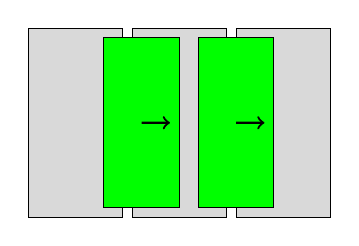
\begin{tikzpicture}[scale=1.2]

\coordinate (A) at (0,2.1);
\coordinate (B) at (1.1,2.1);
\coordinate (C) at (2.2,2.1);


\foreach \v in {A,B,C}
{
    \draw[fill=gray!30] (\v) + (-0.5,-1) rectangle ++(0.5, 1);
}

\coordinate (D) at (0.7, 2.1);
\coordinate (E) at (1.7, 2.1);

\foreach \v in {D,E}
{
    \draw[fill=green] (\v) + (-0.4,-0.9) rectangle ++(0.4, 0.9);
}

\draw[thick,black,->] (D) -- (1,2.1);
\draw[thick,black,->] (E) -- (2,2.1);

\end{tikzpicture}

        \caption{Green rectangles are robots and gray rectangles are parking
            spaces. Both robots are moving in the same direction without a
            collision as long as the left robot is not moving faster then the right
        one.}
        \label{fig:simumove}
    \end{center}
\end{figure}

\testImage{movetogether}{Initial node statuses for simultaneous movement test.}
Both robots are forced to move at the start by following constraints.
\begin{align}
    \go_{(1,0),\stat{r},\Dw,0} &= 1\\
    \go_{(2,0),\stat{r},\Dw,0} &= 1
\end{align}
The model should be feasible and a feasible solution is also verified by following
checks, which should hold for all feasible solutions.
\begin{align}
    \nstat_{(0,0), \stat{r}, 2} &\ife 1\\
    \nstat_{(1,0), \stat{r}, 2} &\ife 1\\
    \nstat_{(2,0), \stat{e}, 2} &\ife 1
\end{align}

\subsubsection{Simultaneous movement II}
This is quite similar to last test, but now we have other than empty nodes in
the way and one of the robots is also carrying a car. All the robots are forced
to start moving to $\Dw$ by following constraints.
\testImage{movetogetherdiff}{Initial node statuses for simultaneous movement
    test with a car on the way and the last robot carrying a car.}
\begin{align}
    \go_{(1,0),\stat{r},\Dw,0} &= 1\\
    \go_{(2,0),\stat{r},\Dw,0} &= 1\\
    \go_{(3,0),\stat{r},\Dw,0} &= 1\\
    \go_{(4,0),\stat{0r},\Dw,0} &= 1
\end{align}
The model should be feasible and optimal solution is verified by following
checks, which verify that node statuses after movement are correct.
\begin{align}
    \nstat_{(1,0), \stat{r1}, 2} &\ife 1\\
    \nstat_{(1,0), \stat{r}, 2} &\ife 1\\
    \nstat_{(2,0), \stat{r0}, 2} &\ife 1\\
    \nstat_{(3,0), \stat{0r}, 3} &\ife 1\\
    \nstat_{(4,0), \stat{e}, 3} &\ife 1
\end{align}

\subsubsection{Invalid simultaneous movement}
This test checks if node statuses are handled correctly when robots move
side-by-side.
\testImage{movetogetherbad}{Initial node statuses for simultaneous
    movement test with an invalid node status constraint.}
We force simultaneous movement and an invalid node status after the movement
with these constraints.
\begin{align}
    \go_{(1,0),\stat{r},\Dw,0} &= 1\\
    \go_{(2,0),\stat{r},\Dw,0} &= 1\\
    \nstat_{(1,0),\stat{r0},2} &= 1
\end{align}
The status of node $(1,0)$ after the movement, at timestep 2 should
be~$\stat{r}$. However, we give a constraint which should make the model
infeasible.
\subsubsection{Lift and move}
This test checks, if the model can find a correct solution to a simple problem.
\testImage{liftandmove}{Initial node statuses for the lift and move test.}
This time instead of adding constraints to force some actions, we define the
objective function. The objective is to get a robot and a car labeled 0 to node
$(0,0)$ as soon as possible.
\begin{align}
    \min \sum_{t \in \T} -\nstat_{(0,0), \stat{r0}, t}
\end{align}
Correct solution would be for the robot to move into the middle node $(1,0)$,
lift the car from there and carry it to $(0,0)$ and finally drop it there. The
model should be feasible and solution is checked against the following
conditions.
\begin{align}
    \nstat_{(0,0), \stat{e}, 2} &\ife 1\\
    \nstat_{(1,0), \stat{r0}, 2} &\ife 1\\
    \nstat_{(2,0), \stat{0}, 2} &\ife 1\\
    \nstat_{(1,0), \stat{0r}, 8} &\ife 1\\
    \nstat_{(0,0), \stat{0r}, 11} &\ife 1\\
    \nstat_{(0,0), \stat{r0}, 13} &\ife 1
\end{align}
These conditions just make sure that node statuses at various timesteps are
correct.
\subsubsection{Lift and move forced}
This test is almost the same as previous, but now the decisions are forced with
the following constraints.
\testImage{liftandmoveforced}{Initial node statuses for the forced lift and move test.}
\begin{align}
    \go_{(2,0),\stat{r},\Dw,0} &= 1\\
    \lift_{(1,0),\stat{r1},2} &= 1\\
    \go_{(1,0),\stat{1r},\Dw,8} &= 1\\
    \nstat_{(0,0),\stat{e},8} &= 1
\end{align}
The objective is now to issue as many lifts at node $(0,0)$ for car with label 1
as possible.
\begin{align}
    \min \sum_{t \in \T} -\lift_{(0,0), \stat{r1}, t}
\end{align}
The solution is checked against these conditions.
\begin{align}
    \nstat_{(0,0), \stat{e}, 2} &\ife 1\\
    \nstat_{(1,0), \stat{r1}, 2} &\ife 1\\
    \nstat_{(2,0), \stat{0}, 2} &\ife 1\\
    \nstat_{(1,0), \stat{1r}, 8} &\ife 1\\
    \nstat_{(0,0), \stat{1r}, 11} &\ife 1
\end{align}
When the previous test failed, the model did found some infeasible movement to
obtain a better objective value. This test was added to see, if a legal
sequence of decisions was indeed feasible and we have not accidentally over constrained the
model.
\subsubsection{Persistence, no robots}
This test is to make sure that node statuses stay the same when there are no
robots.
\testImage{persistence}{Initial node statuses for the persistence test.}
We also add one odd constraint.
\begin{align}
    \nstat_{(0,0),\stat{r},20} &= 1
\end{align}
And the objective function used encourages the model to occupy edges and
make robots appear.
\begin{align}
    \min \sum_{t \in \T}\left( -4\nstat_{(0,0), \stat{r}, t}
    -4\nstat_{(1,0),\stat{r},t} -\sum_{e \in \E} \occu_{e,t} \right)
\end{align}
Of course node statuses should not change by themselves, and the model should be
infeasible.

\subsubsection{Continue together}
This tests makes sure that robots can continue moving in one direction, even
when moving simultaneously. Actually it tests a single robot continuing and at
the same time also 2 robots continuing simultaneously.
\testImage{largetest}{Initial node statuses for the continue test.}

The objective is for robots to go to the right side.
\begin{align}
    \min \sum_{t \in \T} -\nstat_{(3,0), \stat{r}, t} -\nstat_{(3,1),\stat{r},t} -\nstat_{(2,1),\stat{r},t}
\end{align}
The model should be feasible and the optimal solution is verified by hand.
Valid solution would have robots in the east at the last timestep. And robots
do not stop at intermediate nodes.

\subsection{Constraints}
\label{sec:constraints}
In this section we give the constraints of the integer programming model. Some
of these constraints are redundant, but they might help the solver and they
also provide a meaningful bound for some abbreviations.
\subsubsection{Helper functions and some notations}
\label{sec:helpers}
The first helper function used is $\edg \colon \V \times \D \to \V$. Let
$\edg(v,d)$ denote the node adjacent to $v$ that is in the direction $d$ from node $v$.

For directions we use $d + 1$ to denote the next direction from direction $d$ in
clockwise manner. Logically $d - 1$ is used to mark the next direction from $d$
in counterclockwise manner. For an example: $\Dn + 1 = \De$.

Some decisions take a specified amount of time. We want to disallow making such
decisions, which lead to actions that cannot be completed in the time frame of
the model. For this purpose we want to split $\T$ into two disjoint subsets.
Let $\T_i = \{ t \mid (t+i) \in \T\}$ and $\Tn_i = \T \setminus \T_i$.

The decisions to stop moving or continue moving are mostly used together.
Either one of these implies that node status is about to change. For that
reason we use an abbreviation $\contOrStop_{u,w,d,t} = \cont_{u,w,d,t} +
\stp_{u,w,d,t}$.

Sometimes we need to denote the set of neighbours for a vertex. We use $\N(v)$
to denote the neighbouring vertices of node~$v$.

Depending on the direction and whether the robot is carrying a car, the
movement takes different number of timesteps. For this, we introduce a new
function $\getMT \colon \Wmc \times \D \to \mathbb{N}$. Function $\getMT(w,d)$
returns the number of timesteps the movement of $w$ takes in direction $d$.

For working with node statuses related to moving there is a notion of moving
component, which is the status, that can move. First is when node status
is~$w$, we need to get the status that can move away from $w$, we define
$\getMC \colon \Wm \to \Wmc$ as:
\begin{align}
    &\forall i \in \{0,\ldots,K-1\} \colon &\getMC(\stat{ri}) &= \stat{r}\\
    &\forall i \in \{0,\ldots,K-1\} \colon &\getMC(\stat{ir}) &= \stat{ir}\\
    & &\getMC(\stat{r}) &= \stat{r}
\end{align}
Next we want to know what remained in the node, when moving component was
removed, for that we define function $\remMC\colon: \Wm \to \W$ as:
\begin{align}
    &\forall i \in \{0,\ldots,K-1\} \colon &\remMC(\stat{ri}) &= \stat{i}\\
    &\forall i \in \{0,\ldots,K-1\} \colon &\remMC(\stat{ir}) &= \stat{e}\\
    & &\remMC(\stat{r}) &= \stat{e}
\end{align}
And sometimes when a moving component comes into node with some status, we want
to know what will the new status will be. We define a partial function $\addMC
\colon \W \times \Wmc \to \W$ as:
\begin{align}
    &\forall i \in \{0,\ldots,K-1\} \colon &\addMC(\stat{e},\stat{ir}) &=
    \stat{ir}\\
    &\forall i \in \{0,\ldots,K-1\} \colon &\addMC(\stat{i},\stat{r}) &=
    \stat{ri}\\
    & &\addMC(\stat{e},\stat{r}) &= \stat{r}
\end{align}

\subsubsection{Simple constraints}
\label{sec:simple}
First constraint is to make sure that at every timestep each node has exactly
one status variable set.
\begin{align}
    &\forall v \in \V \colon \forall t \in \T \colon & \sum_{w \in \W}
    \nstat_{v,w,t} = 1
\end{align}
When a directed edge is used, its opposite cannot be used at the same time.
\begin{align}
    &\forall (u,v) \in \E \colon \forall t \in \T \colon & \occu_{(u,v),t} +
    \occu_{(v,u),t} \leq 1
\end{align}
No more than one moving thing can arrive at the same node at the same time.
\begin{align}
    \label{eq:edgedest}
    &\forall v \in \V \colon \forall t \in \T \colon & \sum_{u \in \N(v)}
    \occu_{(u,v),t} \leq 1
\end{align}
We also want to forbid movements in the orthogonal directions.
\begin{equation}
    \begin{split}
        \label{eq:edgeorth}
        \forall v \in \V \colon \forall d \in \D \colon \forall t \in \T \colon
        \quad & \occu_{(\edg(v,d),v),t} \\ + \occu_{(v,\edg(v,d-1)),t} + &
        \occu_{(v,\edg(v,d+1)),t} \leq 1
    \end{split}
\end{equation}
Note that there are vertices such that they do not have an edge between them, or
they do not even have a neighbour in some directions. When that happens, the
invalid $\occu_{e,t}$ variables are not added to the sums in
constraints~\eqref{eq:edgedest} and~\eqref{eq:edgeorth}.

It does not make sense to allow more than 1 decision at the same time, at
the same location. Only one robot is at one node at one time and it cannot make
two actions at the same time.
\begin{equation}
    \begin{split}
        \forall v \in \V \colon \forall t \in \T \colon \quad & \sum_{d \in \D,
        w \in \Wmc}(\go_{v,w,d,t} + \stp_{v,w,d,t} + \cont_{v,w,d,t}) \\ + &
        \sum_{w \in \Wl} \lift_{v,w,t} + \sum_{w \in \Wd} \drop_{v,w,t} \leq 1
    \end{split}
\end{equation}

\subsubsection{Lifting and dropping constraints}
These constraints describe the lifting and dropping of cars. In fact they are
quite similar, they indeed are opposite actions. We will start with lifting
constraints. Instead of using $\T$, like we did in~\autoref{sec:simple}, we use
$\T_6$, because lifting takes 6 timesteps. First constraint type is to make sure
that the node status is correct, when a decision to lift is made.
\begin{align}
    &\forall v \in \V \colon \forall w \in \Wl \colon \forall t \in \T_6 \colon
    &\lift_{v,w,t} - \nstat_{v,w,t} \leq 0
\end{align}
While the lifting is in progress, we want the node status be fixed to
$\stat{lft}$.
\begin{align}
    &\forall v \in \V \colon \forall w \in \Wl \colon \forall t \in \T_6 \colon
    \forall i \in \{1,\ldots,5\} \colon &\lift_{v,w,t} -
    \nstat_{v,\stat{lft},t+i} \leq 0
\end{align}
And at the end of lifting, the node status should correspond to the lifted
thing. For that we have a simple bijective helper function $f \colon \Wl \to \Wd$. It is
defined as: $\forall i \in \{0,\ldots,K-1\} \colon f(\stat{ri}) = \stat{ir}$.
In words, the function $f$ determines the node status after lifting. By using
$f$ we can now give the constraints, which determine the node status after
lifting.
\begin{align}
    &\forall v \in \V \colon \forall w \in \Wl \colon \forall t \in \T_6 \colon
    &\lift_{v,w,t} - \nstat_{v,f(w),t+6} \leq 0
\end{align}
If the lifting cannot be completed, we just make sure that the decision is
never made. As a reminder $\Tn_6$ is the set timesteps for which adding 6 more
timesteps would be more that $t_{\max}$, and therefore be outside the scope of
the model.
\begin{align}
    &\forall v \in \V \colon \forall w \in \Wl \colon \forall t \in \Tn_6
    \colon &\lift_{v,w,t} = 0
\end{align}

For dropping we have almost the same constraints. First make sure that the node
status is correct, when decision is made.
\begin{align}
    &\forall v \in \V \colon \forall w \in \Wd \colon \forall t \in \T_2 \colon
    &\drop_{v,w,t} - \nstat_{v,w,t} \leq 0
\end{align}
Dropping takes less time than lifting, therefore the constraints for
intermediate node state are simpler than for lifting.
\begin{align}
    &\forall v \in \V \colon \forall w \in \Wd \colon \forall t \in \T_2 \colon
    &\drop_{v,w,t} - \nstat_{v,\stat{drp},t+1} \leq 0
\end{align}
To get the correct node status at the end of the drop, we can use the inverse
of the previous helper function $f$.
\begin{align}
    &\forall v \in \V \colon \forall w \in \Wd \colon \forall t \in \T_2 \colon
    &\drop_{v,w,t} - \nstat_{v,f^{-1}(w),t+2} \leq 0
\end{align}
As with lifting, if dropping action cannot be completed in the time frame of
the model, disable the decision.
\begin{align}
    &\forall v \in \V \colon \forall w \in \Wd \colon \forall t \in \Tn_2
    \colon &\drop_{v,w,t} = 0
\end{align}

\subsubsection{Moving constraints}
While constructing movement constraints, we need some abbreviations and cannot
write all the quantifiers before every constraint. Therefore, the constraints
in this section are for all combinations of $u \in \V$, $w \in \Wmc$, $d \in
\D$ and $t \in \T$. \TODO{Fix this paragraph}

Now let $\td = \getMT(w,d)$, and $\td' = \td-1$. When movement starts at time $t$,
the node status will change at time $t+\td$, and at time $t+\td'$ a decision
has to be made to continue moving in the same direction or stop. Let $v =
\edg(u,d)$ be the destination node and $e = (u,v)$ the edge that is used for
movement. Later we also need $u' = \edg(u,d+2)$\footnote{$d+2$ means the
opposite direction from $d$}, which is the node before $u$ and $v' =
\edg(v,d)$, which is the node after $v$. It might be easier to look at an
example on~\autoref{fig:upuvvp}.

\begin{figure}[h]
    \begin{center}
        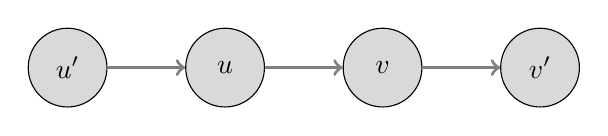
\begin{tikzpicture}
\tikzstyle{every node}=[draw,fill=gray!30,shape=circle, minimum size=1cm];
\node (up) at (0,0) {$u'$};
\node (u) at (2,0) {$u$};
\node (v) at (4,0) {$v$};
\node (vp) at (6,0) {$v'$};
\draw[very thick,gray,->] (up) edge (u) (u) edge (v) (v) edge (vp);
\end{tikzpicture}

        \caption{Illustration for the meanings of $u',u,v,v'$. The arrows show
        the direction $d$.}
        \label{fig:upuvvp}
    \end{center}
\end{figure}

Also we need the set of node statuses where the moving component $w$ could come
from.
\begin{align}
    \uw = \{w_m \mid w_m \in \Wm \wedge \getMC(w_m) = w\}
\end{align}
When $e \notin \E$ we skip the constraints, because we do not have movement
variables for such a combination of starting vertex $u$ and direction $d$. By
skipping the constraints we mean that we do not add the remainder of the
constraints in this section for current values of $(u,w,d,t)$ and we
immediately go to next combination of $(u,w,d,t)$. Also when $t+\td' \notin \T$
we disable the start of movement, because it cannot be finished.
\begin{align}
    \label{eq:gotime}
    &\IF{t+\td' \notin \T} &\go_{u,w,d,t} = 0
\end{align}
In addition to disabling go, we skip the rest of the constraints.

As with other decisions the first group of constraints make sure that node
status is correct at the time of the decision. In this case it has to be one of
the possible node statuses in $\uw$.
\begin{align}
    & \go_{u,w,d,t} - \sum_{w_u \in \uw} \nstat_{u,w_u,t} \leq 0
\end{align}
If we have the edge $(u',u) \in \E$, that means that an already moving object
could continue moving from $u'$ and is in other ways equivalent to a moving
object, that starts accelerating from $u$. So we define an abbreviation.
\begin{align*}
    \goOrCont = \begin{cases}
        \go_{u,w,d,t} \IFc (u',u) \notin \E\\
        \go_{u,w,d,t} + \cont_{u',w,d,t} \IFc (u',u) \in \E
    \end{cases}
\end{align*}
We also give a constraint to make sure that these things do not happen at the
same time.
\begin{align}
    \goOrCont \leq 1
\end{align}
When there is movement, it has to be continued or stopped.
\begin{align}
    \label{eq:goImpcont}
    \goOrCont - \stp_{u,w,d,t+\td'} - \cont_{u,w,d,t+\td'} = 0
\end{align}
Now again we have to check if movement can actually be completed. Earlier we
checked if $t+\td' \notin \T$ and skipped the rest of the constraints. However
now we check for $t+\td \not \T$. When that happens, we again disable the
movement like in constraint~\eqref{eq:gotime}.
\begin{align}
    &\IF{t+\td' \notin \T} &\go_{u,w,d,t} = 0
\end{align}
And skip the rest of the constraints. At first this seems redundant, but we
need to do it like this, because otherwise constraint~\eqref{eq:goImpcont} would
not exist for $\cont$ and $\stp$ variables at the last timestep and no
constraint would stop them from obtaining value 1.

For the duration of movement the edge $e$ must be occupied and the node status
should remain same. However from $w$, we do not know the actual status of $u$,
therefore we have to go through all possibilities.
\begin{align}
    \forall i \in \{0,\ldots,\td'\}\colon \  \goOrCont - \occu_{e,t+i} &\leq 0\\
    \forall i \in \{1,\ldots,\td'\}\colon \forall w_u \in \uw\colon \ \goOrCont
    + \nstat_{u,w_u,t} - \nstat_{u,w_u,t+i} &\leq 1
\end{align}
There is a simple check: if edge $(v,v') \notin \E$, we can disable continue at
$u$, because after reaching $v$ the robot cannot continue to $v'$. Also when
$t$ is so small, that a previous continue or go decision could not be made, we
disable both the stop and continue at time $t$.
\begin{align}
    &\IF{(v,v') \notin \E} &\cont_{u,w,d,t+\td'} = 0\\
    &\IF{t < \td'} &\cont_{u,w,d,t} = 0\\
    &\IF{t < \td'} &\stp_{u,w,d,t} = 0
\end{align}
Specifying node statuses for $u$ and $v$ after the movement would be simpler,
if things could not move simultaneously side-by-side as
on~\autoref{fig:simumove}. However robots can move side-by-side, at the same
direction. For that reason we need to define additional set of node statuses
and corresponding variables. When the robot moves away from $u$, another thing
can at the same time come from~$u'$ into~$u$. For that purpose, we define the
set of statuses, that can move behind~$w$ as $\B$. At the same time another
moving object can disappear from~$v$ to~$v'$. Let $\A$ denote the set of things that
can move ahead of~$w$.
\begin{align}
    &\B = \begin{cases}
        \Wmc \IFc w = \stat{r}\\
        \Wd \IFc w \neq \stat{r}
    \end{cases}
    &\A = \begin{cases}
        \{\stat{r}\} \IFc w = \stat{r}\\
        \Wmc \IFc w \neq \stat{r}
    \end{cases}
\end{align}
Now we construct the set of variables, which imply that some additional object
is coming into $u$. Also now is the time to use the abbreviation $\contOrStop$,
as a reminder it was defined as $\contOrStop_{u,w,d,t} = \cont_{u,w,d,t} +
\stp_{u,w,d,t}$.
\begin{align}
    \um = \begin{cases}
        0 \IFc (u',u) \notin \E\\
        \sum_{w_{u'} \in \B} \contOrStop_{u',w_{u'},d,t+\td'} \IFc (u',u) \in
        \E
    \end{cases}
\end{align}
Now we can give the general constraint, which says something about $u$ status
at the end of movement. When $w$ moves away from $u$, it's status should be the
beginning status minus the $w$, or something else must have come into $u$. To
get the beginning status without $w$ we can use the helper function $\remMC$,
which removes a moving component from node status.
\begin{align}
    \contOrStop_{u,w,d,t+\td'} -\sum_{w_u \in \uw}\nstat_{u,\remMC(w_u),t+\td}
    -\um \leq 0
\end{align}
The last constraint was a general one, that did not exactly specify the status
of $u$ after movement. To actually specify the status of $u$ after movement, we
need to go over all possible $w_u \in \uw$. When $u$ status is about to change
by continuing or stopping, and the $u$ status was $w_u$, the new status should
be $\remMC(w_u)$\footnote{$w_u$ without the moveable component} or something
else moved at the same time into $u$.
\begin{align}
    \begin{split}
        \forall w_u \in \uw\colon\quad \contOrStop_{u,w,d,t+\td'}
        - \um &+ \nstat_{u,w_u,t+\td'}\\ &-\nstat_{u,\remMC(w_u),t+\td'} \leq 1
    \end{split}
\end{align}
Only when there the edge $(u\,u)$ exists in $\E$, the following group of
constraints is added. These make sure that if $w_b \in \B$ moved from $u'$ to $u$
the new status of $u$ will be what would be left in $u$ plus the thing that
moved in. 
\begin{align}
    \begin{split}
        \label{eq:addmove}
        \forall w_u \in \uw\colon &\forall w_b \in \B\colon \quad
        \cont_{u',w_b,d,t+\td'} + \stp_{u',w_b,d,t+\td'}\\
        &+\nstat_{u,w_u,t+\td'}
        -\nstat_{u,\addMC(\remMC(w_u), w_b),t+\td} \leq 1
    \end{split}
\end{align}
There are some subtle details hidden here: when the thing left in $u$ is a car
and a robot carrying another car comes. In that case the function $\addMC$ is
undefined, and the constraint~\eqref{eq:addmove} for that combination of~$w_u$ and~$w_b$ is not
added.

Now we want to say something about $v$ status at the end of movement. For that
we use the set of statuses that are possible for $v$ after $w$ has moved into
it. It turns out that the set is exactly $\uw$, which contained all the
possible node status from where movement could originate from. Movement implies
that at the end $v$ has one of statuses in $\uw$.
\begin{align}
        \contOrStop_{u,w,d,t+\td'} -\sum_{w_v \in \uw}
        \nstat_{v,w_v,t+\td} \leq 0
\end{align}
Similarly to $\um$ we construct the set of variables, which imply that something is
moving away from $v$.
\begin{align}
    \vl = \begin{cases}
        0 \IFc (v,v') \notin \E\\
        \sum_{w_v \in \A} \contOrStop_{v,w_v,d,t+\td'} \IFc (v,v') \in \E
    \end{cases}
\end{align}
Now we go over all possible status that $v$ could have at the end of the
movement and specify the actual status. If the end status of $v$ is $w_v$ then
status of $v$ was $\remMC(w_v)$ or something moved away from $v$.
\begin{align}
    \begin{split}
        \forall w_v \in \uw\colon \quad
        \contOrStop_{u,w,d,t+\td'}
        &-\nstat_{v,\remMC(w_v),t+\td'}\\
        &+\nstat_{v,w_v,t+\td} -\vl \leq 1
    \end{split}
\end{align}
\subsubsection{Node status constraints}
Purpose of node status constraints is to make sure that node statuses remain
unchanged when no movement occurs. As with moving constraints, we declare that
the remainder of the section is applied to all possible combinations of $u \in
\V$, $w \in \W$ and $t \in \T_1$.

The basic idea is to list all variables that could change the status of $u$
between timesteps $t$ and $t+1$. We define a lot of sets and then finally use
the union of them. First are the lift and drop variables for the
current timestep~$t$.
\begin{align}
    &\A_{\mathrm{lift}} = \begin{cases}
        \{\lift_{u,w,t}\} \IFc w \in \Wl\\
        \emptyset \IFc w \notin \Wl
    \end{cases}
    &\A_{\mathrm{drop}} = \begin{cases}
        \{\drop_{u,w,t}\} \IFc w \in \Wd\\
        \emptyset \IFc w \notin \Wd
    \end{cases}
\end{align}
Next are the lift and drop variables that happened in the past.
\begin{align}
    \B_{\mathrm{lift}} &= \begin{cases}
        \{\lift_{u,w_l,t-5} \mid w_l \in \Wl\} \IFc w = \stat{lft} \wedge
        t \in \T_{-5}\\
        \emptyset \IFco
    \end{cases}\\
    \B_{\mathrm{drop}} &= \begin{cases}
        \{\drop_{u,w_d,t-1} \mid w_d \in \Wd\} \IFc w = \stat{drp} \wedge
        t \in \T_{-1}\\
        \emptyset \IFco
    \end{cases}
\end{align}
Now there are the movement variables. Only continue and stop variables actually
correspond to immediate node status changes.
\begin{align}
    \A_{\mathrm{move}} &= \begin{cases}
        \{\contOrStop_{u,\getMC(w),d,t} \mid d \in \D \wedge (u,\edg(u,d)) \in \E\} \IFc
         w \in \Wm\\
        \emptyset \IFco
    \end{cases}
\end{align}
We use $\B_{\mathrm{move}}$ to denote all the movements that could come
into~$u$. The expression $\addMC(w,w_m) = \emptyset$ holds, when $w_m$ could
not be added to $w$.
\begin{align}
    \begin{split}
    \B_{\mathrm{move}} =
    \{\contOrStop_{\edg(u,d),w_m,d+2,t} &\mid d \in \D,  w_m \in \Wm\\
        &\wedge \addMC(w,w_m) \neq \emptyset \wedge  (\edg(u,d),u) \in \E\}
    \end{split}
\end{align}
Now that we have defined all the subpart we join them together.
\begin{align}
    \B &= \B_{\mathrm{lift}} \cup \B_{\mathrm{drop}} \cup \B_{\mathrm{move}} \\
    \A &= \A_{\mathrm{lift}} \cup \A_{\mathrm{drop}} \cup \A_{\mathrm{move}}
\end{align}
Now we can finally give the constraints. The following constraints say that
only one action from the set of node status changing actions can happen at
once. There are two sets, because with simultaneous movement, it can happen
that one action is for moving away and another for moving into~$u$.
\begin{align}
    \sum_{b \in \B} b \leq 1\\
    \sum_{a \in \A} a \leq 1
\end{align}
When node status for~$u$ is~$w$, the node status has to remain same or some
kind of action must have changed it.
\begin{align}
    \nstat_{u,w,t} - \nstat_{u,w,t+1} -\sum_{b \in \B} b -\sum_{a \in \A} a
    \leq 0
\end{align}
If node status in the future is~$w$ and something came into the node, another
thing must have left the node~$u$.
\begin{align}
    \nstat_{u,w,t+1} +\sum_{b \in \B} b -\sum_{a \in \A} a
    \leq 1
\end{align}
\subsubsection{Edge occupied constraints}
These constrains are to make sure, that when no movement is using an edge the
edge occupied variable will be 0. Constraints in this section are applied for
all combinations of $e=(u,v) \in \E$ and $t \in \T$.
Let $d=\dir(e)$ denote the direction of edge $e$. First we collect all variables
which imply that edge is occupied.
\begin{align}
    \A = \{\cos_{u,w,d,t+\td'} \mid w \in \Wmc, \td' \in
    \{0,\ldots,\getMT(d,w)-1\} \wedge t+\td' \in T\}
\end{align}
At most two of movement
variables in $\A$ can be 1. The reasoning is that at time $t$ an object moves
away from $u$ but at the end of the movement ($t+\td'$) another object which
entered $u$ at time $t$ could also leave it. This happens only when two robots
are simultaneously moving side-by-side and continuing to move.
\begin{align}
    \A \leq 2
\end{align}
We would want an equality constraint $\occu_{e,t} - \sum_{a \in \A} a = 0$
which would tell us that, edge is occupied when movement implied it, and
movement occurs, when edge is occupied. However, $\occu_{e,t}$ is a binary
variable, but $\A$ is not and can also obtain value 2, therefore we need to
simulate the equality constraint with two inequality constraints.
\begin{align}
    \occu_{e,t} - \sum_{a \in \A}a &\leq 0\\
    2\occu_{e,t} - \sum_{a \in \A}a &\geq 0
\end{align}
\subsection{Initial status and objective}
\newcommand{\initW}[1]{\bar{#1}}
\newcommand{\termW}[1]{\hat{#1}}
Initial status will be fixed by adding constraints. Let the initial status of
node $v$ be denoted by $\initW{v}$, then we can add constraints to fix node
status variables at the first timestep.
\begin{align}
    &\forall v \in \V\colon &\nstat_{v,\initW{v},0} = 1
\end{align}
Let $\termW{v}$ denote the end status of node $v$. There are different ways to make
the model find a solution. One way is to add constraints for the last timestep.
\begin{align}
    \label{eq:termcont}
    &\forall v \in \V\colon &\nstat_{v,\termW{v},t_{\max}} = 1
\end{align}
We still have not defined the objective function to the model. We can
define the objective function in a way that we do not need the constraints for
the end status.
\begin{align}
    \min \sum_{v \in \V,t \in \T} -\nstat_{v,\termW{v},t}
\end{align}
This objective means that for every node~$v$, we want the status be~$\termW{v}$
for as long as possible or in other words, as soon as possible.

Other possible objective functions can be considered. Maybe it does not make
sense to add all node statuses to objective. If we ignore the empty nodes, we
can decrease the number of variables in the objective.
\begin{align}
    \label{eq:timeobj}
    \min \sum_{v \in \V,t \in \T,\termW{v} \neq \stat{e}}
    -\nstat_{v,\termW{v},t}
\end{align}
However this is objective does not actually minimize the time needed to move
everything to final positions. A robot might go to its destination instead of
first moving the car, because that might get a better objective. An example can
be found at~\autoref{apx:movement}.

Sometimes the optimal solution consist of one robot waiting for other to move
out of way. Instead of standing still, the waiting robot moves back and forth.
This is undesired behaviour of the model, because it wastes energy. Therefore
another possible objective function would be to use the end status constraints
and then minimize energy used.
\begin{align}
    \begin{split}
        \label{eq:energyobj}
        \min \sum_{e=(u,v) \in \E,w \in \Wmc,t \in \T}
        &C_{1,w} \go_{u,w,\dir(e),t} + C_{2,w} \cont_{u,w,\dir(e),t} + C_{3,w}
        \stp_{u,w,\dir(e),t}\\
        +\sum_{v \in \V, w \in \Wl,t \in \T} &D_{1,w} \lift_{v,w,t}
        +\sum_{v \in \V, w \in \Wd,t \in \T} D_{2,w} \drop_{v,w,t}
    \end{split}
\end{align}
Here $C$ is $(3 \times |\Wmc|)$-dimensional matrix that contains the amount of
energy used by the movement. For lifting and dropping we have a similar matrix
$D$. That way we can give different costs to different to every action and even
to every labeled car. This would give optimal solutions energy-wise,
but we are more concerned about time.

Therefore, a combination of both~\eqref{eq:energyobj} and \eqref{eq:timeobj}
might be the better. After testing such a combination, it turned out that the
problem of robot moving to destination before doing any work was still the
case, however it removed the problem of robots doing unnecessary
actions instead of waiting.

The next objective function was to minimize energy, but actions at later
timesteps would cost more. And also give a penalty if at $t_{\max}$, the node
status is different from terminal state~$\termW{v}$. Let $g(t) = 1 +
\frac{t}{t_{\max}}$.
\begin{align}
    \begin{split}
        \label{eq:objective}
        \min \sum_{(u,v) \in \E,w \in \Wmc,t \in \T,d=\dir((u,v))}(0.2 g(t) \cdot
        \go_{u,w,d,t} + 0.1 g(t) \cdot \cont_{u,w,d,t}\\ + 0.2 g(t)
        \cdot \stp_{u,w,d,t})
        +\sum_{v \in \V, w \in \Wl,t \in \T} 0.4 g(t) \cdot \lift_{v,w,t}\\
        +\sum_{v \in \V, w \in \Wd,t \in \T} 0.1 g(t) \cdot \drop_{v,w,t}\\
        +\sum_{v \in \V, w \in \W, w \neq \termW{v}} 10 \cdot
        \nstat_{v,w,t_{\max}}
    \end{split}
\end{align}

In the end we used objective function~\eqref{eq:objective} with a small
modification to only give penalties to those node statuses, where the terminal
status contains a labeled car.

It should also be mentioned that the model performance varied greatly with
different objective functions. And also on the fact, if terminal configuration
is set with constraints or not.

\subsection{Size of the model}
It is customary to give the total number of variables, equalities and
inequalities for a integer programming model. In our case these numbers are
dependant of the exact graph~$\mathcal{G}=(\V,\E)$, number of different labels for
cars~$K$, and the number of timesteps~$t_{\max}$. Because $|\T| = \tm + 1$, we
use $|\T|$ in further calculations. We use abbreviations $T = |\T|, V
= |\V|$ and $E = |\E|$.

We first give the sizes of $\W, \Wl, \Wd, \Wm$ and $\Wmc$.
\begin{align}
    |\W| &= 4 + 3K\\
    |\Wl| &= K\\
    |\Wd| &= K\\
    |\Wm| &= 1 + 2K\\
    |\Wmc| &= 1 + K
\end{align}
\subsubsection{Number of variables}
\label{sec:numv}
We start with node status variables.
\begin{align}
    VWT = V(4 + 3K)T = TV(3K + 4)
\end{align}
The number of edge variables is $ET$.
The number of decision variables is:
\begin{align}
    \begin{split}
        3E\Wmc\T &+ V|\Wl|T + V|\Wd|T\\
        &= T(3E|\Wmc| + V(|\Wl| + |\Wd|))\\
        &= T(3E(1+K) + 2VK)
    \end{split}
\end{align}
Total number of variables is:
\begin{align}
    \begin{split}
        TV(3K+4) &+ ET + T(3E(1+K) + 2VK)\\
        &= T(V(3K+4) + E + 3E(1+K) + 2VK)\\
        &= T(5VK + 3EK + 4V +4E)
    \end{split}
\end{align}
\subsubsection{Number of equalities}
We have only two groups of real equality constraints. The others are meant to
fix a value of a variable, and therefore we do not count them here. Although
those variables will be fixed by equality constraints, We still counted them
in~\autoref{sec:numv}.
Total number of equality constraints is $TV + TE(1+K)= T(EK + E + V)$.
\subsubsection{Number of inequalities}
There are lots of inequalities so we will not give an exact number, but an
upper bound.
From simple constraint and lifting constraints the number of inequalities is:
\begin{align}
    \begin{split}
        TE + TV + 4TV &+ TV + TVK + 5TVK + TVK + TVK + TVK + TVK\\
        &=10TVK + 6TV + TE
    \end{split}
\end{align}

From moving constraints we get the following upper bound on number of
inequalities:
\begin{align}
    \begin{split}
        TE(1+K)(1 + 1 &+ 5 + 5K + 1 + K + K^2 + 1 + K)\\
        &=TE(1+K)(K^2 + 7K + 9)
    \end{split}
\end{align}

For node status constraints the upper bound on inequalities is:
\begin{align}
    TV(4+3K)(1 + 1 + 1 + 1) = 12TVK + 16TV
\end{align}
For edge occupied constraint the upper bound is: $TE(1+1+1) = 3TE$.

In total the upper bound of inequalities is:
\begin{align}
    \begin{split}
        10TVK &+ 6TV + TE + TE(1+K)(K^2 + 7K + 9) + 12TVK + 16TV + 3TE\\
        &= 22TVK + 22TV + 4TE + (TE + TEK)(K^2 + 7K + 9)\\
        &= 22TVK + 22TV + 4TE + TEK^2 + 7TEK + 9TE + TEK^3 + 7TEK^2 + 9TEK\\
        &= TEK^3 + 8TEK^2 + 22TVK + 16TEK + 22TV + 13TE\\
        &= T(EK^3 + 8EK^2 + 22VK + 16EK + 22V + 13E)
    \end{split}
\end{align}
